\subsection{Graphical user interface}
\label{subsec:userGUI}
Easy and prompt access to new and improved data analysis algorithms is essential in many fields of application where the development 
of data analysis algorithms and progress on the application side are deeply linked to each other. \alida meets these requirements 
by providing a mechanism to automatically generate handy graphical user interfaces (GUI) for all operators implemented within its 
framework. 

\subsubsection{Graphical operator runner} 
The operator GUIs can easily be invoked from \alida's graphical operator runner,
named \icode{ALDOpRunnerGUI}, to be found in the package
\icode{de.unihalle.informatik.Ali\-da.tools}. Upon invocation the main window of
the operator runner is shown, from where operators can be selected for
execution. A screenshot of the main window is displayed in Fig.~\ref{fig:OpRunnerGUIMain}.

The main part of the window is formed by the tree view of all available
operators, hierarchically arranged due to their package structure. From this
view the operators to be executed can be chosen. An operator can be invoked by
either double-clicking on its item in the tree, or by selecting the entry with a
single mouse-click and then pressing the \icode{'Configure Operator\ldots'}
button at the bottom of the window. Note that the tree view allows to configure
the set of initially unfolded packages, i.e., visible operators.
To this end the user needs to provide a file with the set of his or her favorite
operators, and set a related environment variable to the name of that file (see
Sec.~\ref{subsec:configure-user} for details). In addition, the operator runner
provides a search and filter function, accessible via the entry field and
filter button in the bottom part of the window. For finding operators with
specific names, type in the name of the operator or a substring of its name,
then press the button or hit the return key. Subsequently the tree will only
contain the operators matching the filter string. Note that the filter function
is not case-sensitive.
  
To further ease operator selection and improve usability of the operator runner,
\alida supports two different categories of operators. The first category of operators is mainly
dedicated to non-expert users and often targets at concrete applications, the
second set additionally subsumes more sophisticated operators often being very
specialized and primarily intended to be used by experts. The tree view of the operator runner
window allows to switch between the first set and a view showing all available operators by
choosing the categories via the item \icode{'Options'} followed by \icode{'Operators to Show'} in
the window's menubar. By selecting \icode{'Default'} the tree view of operators is restricted to
operators of the first category, while selecting \icode{'All'} renders all available operators to be
displayed. Note that the menubar also grants access to \alida's online help and the current version
of \alida being used.

\subsubsection{Operator control window} 
\label{subsubsec:controlWin}
Once an operator has been selected, the corresponding operator control window
pops up (Fig.~\ref{fig:OpControlFrame}).
It allows for configuration and execution of the operator. The window is
subdivided into four parts, i.e., it consists of a menubar, a control
section with a set of buttons at the bottom, a status bar, and the configuration
section with different tabs typically occupying the largest fraction of the
window. 
\begin{figure}[t]
\begin{center}
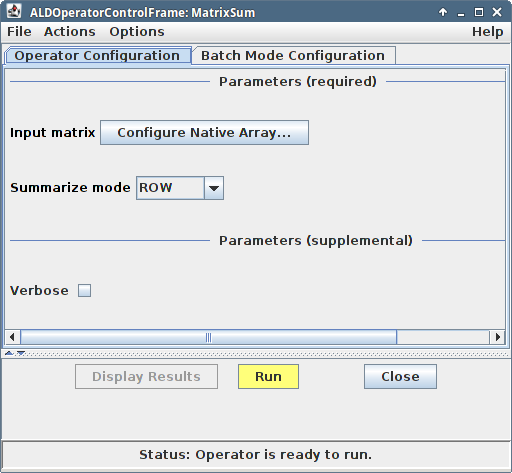
\includegraphics[width=0.5\textwidth]{../images/screenShotOpControlFrame.png}
\caption{\label{fig:OpControlFrame}Automatically generated control window for
the \alida demo operator \icode{MatrixSum}.}
\end{center}
\end{figure}

\vspace*{-0.25cm}
\paragraph{Configuration section.} For most operators there are two tabs
available in the configuration section. The first one, denoted \icode{'Operator
Configuration'}, subsumes graphical elements for handy configuration of the
operator's parameters. As operator parameters may have different data types, and
each data type requires individual I/O handling, with each data type a specific
graphical element is associated. 
For example, for inserting values for native parameters of type \icode{int} or
\icode{double} a simple text field is displayed, while for arrays and
collections buttons are shown which allow to open editable tables. 
The demo operator \icode{MatrixSum} defines the two input parameters
\icode{'Input matrix'} of type \icode{Double[][]} and \icode{'Summarize mode'}.
The latter one is linked to an enumeration class, and a corresponding
combobox for selecting one of the available enumeration elements is shown.
As can be seen from the screenshot in Fig.~\ref{fig:OpControlFrame}, the
configuration section is further subdivided into required and
supplemental parameters. Also optional parameters may appear there, however, the
demo operator in this example does not define any optional parameters, thus, the
corresponding section is missing in this case.

The second tab, denoted \icode{'Batch Mode
Configuration'}, provides access to \alida's built-in support for batch
processing. The basic idea of the batch mode is to automatically execute an
operator multiple times with different input values for a certain parameter.
Consequently, on the tab a single input parameter of the operator can be
selected and configured for batch processing.
In Fig.~\ref{fig:batchConfig} the tab for batch mode configuration of the
operator \icode{ALDArrayMean} is depicted. The operator expects as input an
array of type \icode{Double[]}. After activating the batch mode via the
corresponding checkbox, it is possible to configure this parameter. In this case
the user has to provide an array of type \icode{Double[][]} as input for the
operator\footnote{Note that if the batch mode is activated for a certain
parameter, it is not possible to configure the parameter via the 'Operator
Configuration' tab.} (see Fig.~\ref{fig:batchConfig}).

\begin{center}
\begin{figure}[t]
\begin{center}
\hspace*{-3.0cm}
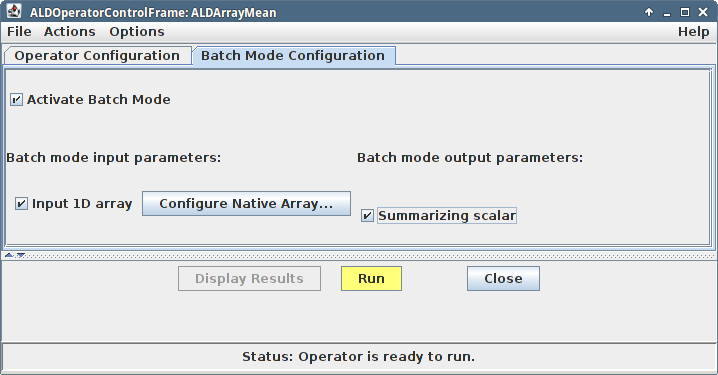
\includegraphics[width=0.7\textwidth]{../images/screenShotALDArrayMeanBatchConfig.png}\\[-1cm]
\hspace*{1cm}
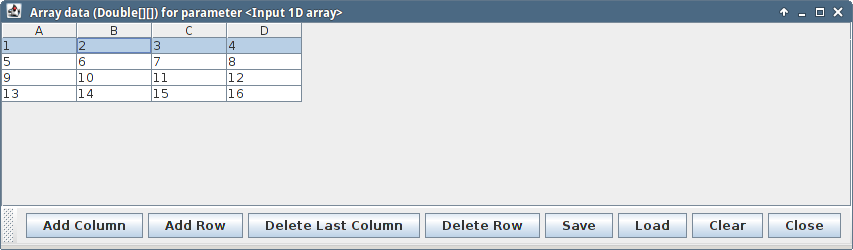
\includegraphics[width=0.75\textwidth]{../images/screenShotALDArrayMeanBatchConfigValues.png}
\vspace*{-0.25cm}
\caption{\label{fig:batchConfig}Screenshot of the tab for batch configuration of
the operator \icode{ALDArrayMean}. As the operator expects as input a 1D array
of type \icode{Double[]} the user has to provide an array of type
\icode{Double[][]} as batch mode input via an appropriate configuration window
(visible at the bottom of this figure).}
\end{center}
\end{figure}
\end{center}

\vspace*{-0.5cm}
During batch processing the operator is run multiple times, each time processing
a single row of the input array (also refer to subsequent paragraph).
The result of such a batch procedure is given by a summary of the values
of selected operator output parameters. The parameters of interest have to be
selected on the batch tab as well, and upon termination of the batch run the
values of the different runs are appropriately summarized
(Fig.~\ref{fig:batchResult}). Note that not all operators allow batch
processing. For these operators the batch mode tab is not shown. The batch mode
support in \alida is in an early state, and currently there is batch support
only for very few input and output parameter data types.
\begin{center}
\begin{figure}[t]
\begin{center}
\hspace*{-2cm}
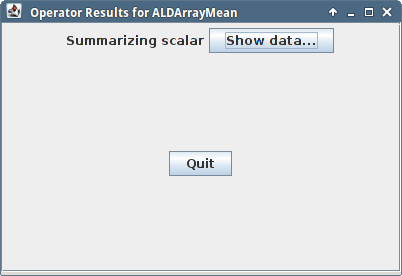
\includegraphics[width=0.4\textwidth,clip,trim=0 0 0 0]
                {../images/screenShotALDArrayMeanBatchResult.png}\\[-2.5cm]
\hspace*{1cm}            
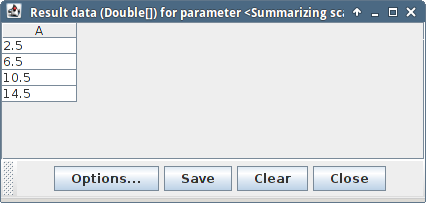
\includegraphics[width=0.4\textwidth,clip,trim=0 0 0 0]
                {../images/screenShotALDArrayMeanBatchResultValues.png}
\caption{\label{fig:batchResult}Window summarizing the batch processing results
for the operator \icode{ALDArrayMean}. Each entry of the result array refers to
the mean of the elements in one row of the batch mode input array
(Fig.~\ref{fig:batchConfig}).}
\end{center}
\end{figure}
\end{center}

\vspace*{-0.5cm}
\paragraph{Control section.} If an operator has been properly configured,
either for normal execution or for batch processing, it can be invoked from the
buttons in the control section of the window. By default, this section contains
a button labeled \icode{'Close'} to close the operator control window, a button
\icode{'Display Results'} (Fig.~\ref{fig:batchConfig}), however, which is
deactivated until results are actually available, and of course a button labeled
\icode{'Run'} to run the operator.
Once the run button is colored yellow, the operator is ready for execution. 
If it has red color, the configuration is not yet completed. A green color
indicates that the operator was already executed with the given set of
parameters and cannot be run again unless the configuration is changed. When the
run button is clicked, \alida executes the operator. While the operator is
running the button takes a blue color. Upon termination its color switches to
green, and a result frame is displayed summarizing the results and also
providing direct access to the input parameters (Fig.~\ref{fig:OpRunnerResult}).

\begin{center}
\begin{figure}[t]
\begin{center}
\hspace*{-3cm}
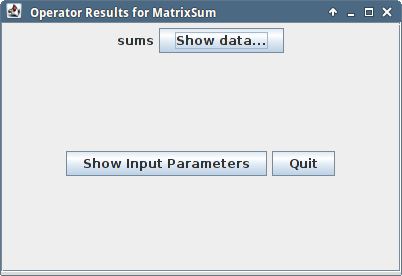
\includegraphics[width=0.45\textwidth,clip, trim= 0 0 0 0]
				{../images/screenShotOpRunnerResult.png}\\[-1.5cm]
\hspace*{5cm}				
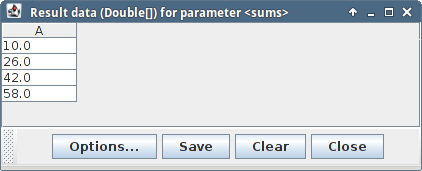
\includegraphics[width=0.45\textwidth,clip, trim= 0 0 0 0]
				{../images/screenShotOpRunnerResultValues.png}
\caption{\label{fig:OpRunnerResult}Result window for the demo operator
\icode{MatrixSum} as displayed upon termination. On the left, the actual result
window is shown, while on the right the result for the operator's output
parameter '\icode{sums}' is displayed, which here is the set of row-wise sums of
the two-dimensional input array. This window pops up by clicking the
\icode{'Show data\ldots'} button in the result frame.}
\end{center}
\end{figure}
\end{center}

\vspace*{-0.75cm}
Besides generic execution of operators in terms of invoking the operator and
displaying its results, \alida also supports interactive operator execution.
Interactive operators allow for user interaction in terms of at least pausing, resuming
or interrupting the data processing. Additionally, interactive operators may also support
step-wise data processing where the operator is automatically paused after a specified number of
steps. The notion of a 'step' in this case is left to the programmer of the individual operator
and may vary between operators. In most cases, however, step-wise execution will be supported
by interactive operators performing several iterations during execution. Each iteration
will then be associated with one execution step. For interactive operators additional control
elements are displayed in the control section of the operator control window
(Fig~\ref{fig:OpControllable}).

\begin{figure}
\begin{center}
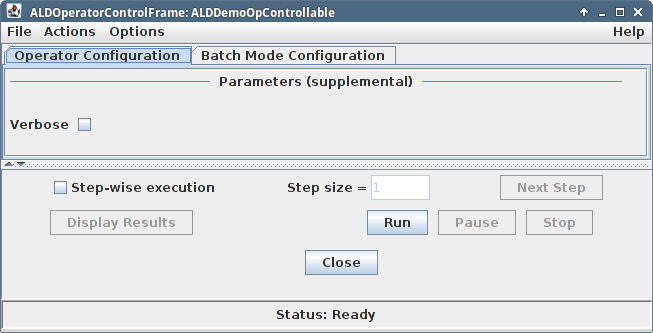
\includegraphics[width=0.6\textwidth]{../images/screenShotOpControllable.png}
\caption{\label{fig:OpControllable}Control window for an operator supporting
interactive execution. Note the set of additional control elements at the bottom
of the window.}
\end{center}
\vspace*{-0.5cm}
\end{figure}
For all interactive operators two additional buttons labeled \icode{'Pause'} and \icode{'Stop'} are
displayed. The execution of an operator has always to be invoked pressing the \icode{'Run'} button.
If the \icode{'Pause'} button is pressed while the execution is ongoing, the operator will be
paused. Note, however, that this does not imply that the operator immediately interrupts its
execution, but rather proceeds until reaching the next {\em breakpoint} predefined by the
programmer. It may even happen that the operator terminates its execution instead of just pausing
it. The latter will be the case if the last breakpoint had been past before the pause command was
triggered by the user. Common breakpoints of operators are for example the end of an iteration in
iterative procedures or the termination of subroutines. In general, however, the definition of a
breakpoint is left to the programmer of an operator and varies between operators. Pressing the
\icode{'Stop'} button during execution triggers a similar behaviour. The operator will proceed
with its execution until the next predefined {\em termination point} is reached, then does some
clean-up and finally presents intermediate results to the user. Termination points may be identical 
to breakpoints, however, this is not mandatory.

If an interactive operator also supports step-wise execution the control windows displays
additional graphical elements to activate the step-wise mode, specify a step size and to trigger
execution of subsequent steps. After activating \icode{'Step-wise execution'} and specifying the step size such an operator
can be invoked by pressing the \icode{'Next Step'} button. The operator then starts its execution
and will automatically pause after the given number of steps. Subsequently the user needs to resume
execution by clicking the button \icode{'Next Step'} again. During step-wise execution the operator
can also directly be terminated by pressing the \icode{'Stop'} button. 
 
\paragraph{Menubar.} The menubar of the operator control window allows for
additional actions. From the menu item \icode{'File'} it is possible to save the
current operator configuration to a file on disk in XML format, and also to load
a configuration from such a file. Note that the batch mode configuration is
currently not included in this file. The \icode{'Actions'} menu offers the possibility to reset
the operator parameters to their default values, and the item \icode{'Options'}
provides access to configuration options for the appearance of the operator control window, e.g., to
switch between different modes of parameter display and to configure the status bar.

Besides defining required, optional and supplemental parameters, \alida supports different modes for
an operator parameter. In detail, a parameter can be declared as \icode{STANDARD} or
\icode{ADVANCED}.
While standard parameters are assumed to be the most important parameters of an operator,
advanced parameters allow for more sophisticated configuration, however, can
most of the time be ignored by non-expert users. Consequently, the parameter
view can configured to show all parameters of an operator or to just display the default set of
most important parameters which is the default setting. 

The item \icode{'Help'} in the menubar again grants access to
Alida's online help.

\paragraph{Status bar.} The status bar at the bottom of each operator control
frame displays the current status of the operator. It tells the user if the operator is
unconfigured, readily configured to be executed, or if it has been executed and result data is
available. In addition, if the underlying operator is triggering progress events during
execution (see Sec.~\ref{subsubsec:implOperators-advanced} for more details),
these can also be displayed in the status bar. The item \icode{'Show Progress Messages'} in the
\icode{'Options'} menu of the menubar allows to enable or disable the display of these messages.
